\documentclass[10pt]{beamer}
\usepackage{ragged2e} % \justifying
\usepackage[export]{adjustbox} % left and right in images
\usetheme{metropolis}           % Use metropolis theme
\title{FP1: Control of the Variable Length Pendulum}
%\subtitle{\textit{Authors:} Xin Xin, Yannian Liu}
\subtitle{Michele Cipriano, Karim Ghonim, Khaled Wahba}
%\date{\today}
\date{}
%\author{Michele Cipriano, Karim Ghonim, Khaled Wahba}
\author{
  \textbf{Control Design and Analysis for Underactuated Robotics:\\
    Variable Length Pendulum}\\
  \textit{Authors:} Xin Xin, Yannian Liu}
\institute{Elective in Robotics: Underactuated Robotics\\
  Department of Computer, Control and Management
  Engineering\\Sapienza University of Rome}

% Fontsize of figure smaller than normalsize:
\setbeamerfont{caption}{size=\scriptsize}

\begin{document}
\nocite{*}

  \maketitle

  \begin{frame}{Introduction}
    \begin{itemize}
      \item Variable Length Pendulum (VLP)
      \item Trajectory Tracking Control
      \item Total Energy Shaping
      \item Partial Energy Shaping
      \item Convergence of Energy
      \item Closed-Loop Equilibrium Points
      \item Simulink
    \end{itemize}
  \end{frame}

  \begin{frame}{Motion Equation}
    \begin{columns}[c,onlytextwidth]
      \column{0.6\textwidth}
        Euler-Lagrange equation:
        \begin{align*}
					&\ddot{\theta}(t)+\frac{2\dot{l}(t)\dot{\theta}(t)}{l(t)}+
						\frac{g\sin\theta(t)}{l(t)} = 0  \\
					&\ddot{l}(t)-ml(t)\dot{\theta}^2(t)-mg\cos\theta(t) = f(t)
				\end{align*}
				Control input:
				\begin{equation*}
					u = \ddot{l}(t)
				\end{equation*}
      \column{0.4\textwidth}
        \begin{figure}
          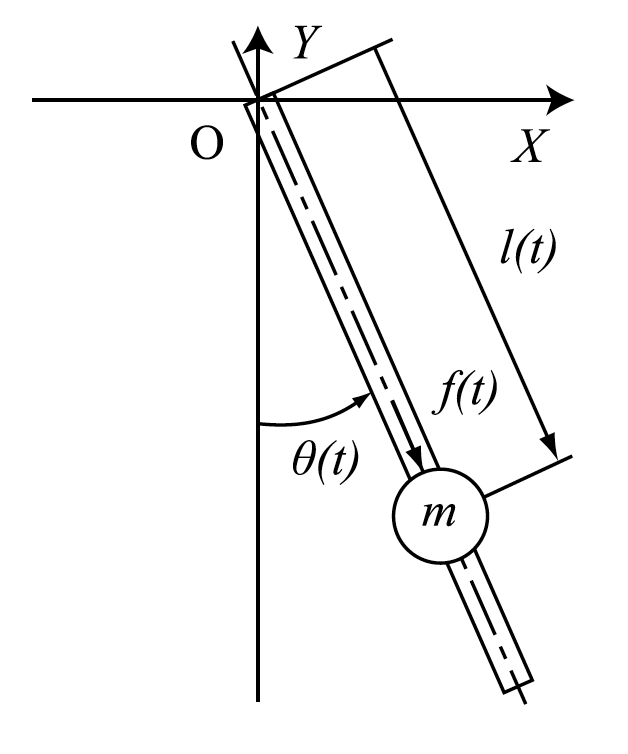
\includegraphics[width=0.96\textwidth,right]{images/vlp.png}
        \end{figure}
    \end{columns}
  \end{frame}

  \begin{frame}{Problem Formulation}
    Let $m=1$. Total mechanical energy:
		\begin{equation*}
      E_T = %T+P =
				\frac{1}{2}\dot{l}^2(t)+\frac{1}{2}\big(l(t)\dot{\theta}(t)\big)^2-
				gl(t)\cos\theta(t) 
    \end{equation*}
		Desired trajectory of swing described by:
		\begin{equation*}
      E_r = \frac{1}{2}\big(l_r\dot{\theta}(t)\big)^2-gl_r\cos\theta(t) 
    \end{equation*}
		with $E_r$ and $l_r$ desired energy and length of the VLP.\\Moreover:
		$E_r = -gl_r\cos\theta_{max}, \theta_{max} \in (0,\pi]$.

		\textbf{Trajectory tracking control problem:}
		\begin{equation*}
			\lim_{t\rightarrow \infty} E_T = E_r  \quad
			\lim_{t\rightarrow \infty} \dot{l} = 0 \quad
		  \lim_{t\rightarrow \infty} l = l_r
		\end{equation*}
  \end{frame}

  \begin{frame}{Controller Design: Total Energy Shaping}
    Lyapunov candidate with $k_P>0$, $k_D>0$:
		\begin{gather*}
			V_c = \frac{1}{2}(E_T-E_r)^2+\frac{1}{2}k_P(l-l_r)^2+
				\frac{1}{2}k_D\dot{l}^2 \\
			\dot{V}_c = \dot{l}\big((E_T-E_r+k_D)u-(E_T-E_r)(l\dot{\theta}^2+
				g\cos\theta)-k_P(l-l_r) \big)
		\end{gather*}
		Controller:
		\begin{equation*}
			u = \frac{(E_T-E_r)(l\dot{\theta}^2+g\cos\theta)-k_P(l-l_r)-
				k_V\dot{l}}{E_T-E_r+k_D}
		\end{equation*}
		with $k_V>0$, then:
		\begin{equation*}
			\dot{V}_c = -k_V\dot{l}^2 \leq 0
		\end{equation*}
		which holds only if:
		\begin{equation*}
			E_T-E_r+k_D  \neq 0 \quad \forall t\geq 0
		\end{equation*}
	\end{frame}

	\begin{frame}{Controller Design: Total Energy Shaping}
		Simulation + Plots.
	\end{frame}

  \begin{frame}{Controller Design: Partial Energy Shaping}
    $E_P$ sum of kinetic energy of rotation and potential energy of VLP:
		\begin{equation*}
			E_P = \frac{1}{2}(l(t)\dot{\theta}(t))^2-gl(t)\cos\theta(t)
		\end{equation*}
		Lyapunov candidate:
		\begin{gather*}
			V = \frac{1}{2}(E_P-E_r)^2+\frac{1}{2}k_P(l-l_r)^2+
      	\frac{1}{2}k_D\dot{l}^2 \\ 
      \dot{V} = \big(-(E_P-E_r)(l\dot{\theta}^2+g\cos\theta)+k_P(l-l_r)\big)
				+ k_D u) \dot{l}
		\end{gather*}
		Controller:
		\begin{equation*}
			u = \frac{(E_P-E_r)(l\dot{\theta}^2+g\cos\theta)-k_P(l-l_r)
        -k_V\dot{l}}{k_D}
		\end{equation*}
		which is free of singular points. Moreover:
		\begin{equation*}
			\dot{V} = -k_V \dot{l}^2 \le 0, \quad k_V > 0
		\end{equation*}
  \end{frame}

	\begin{frame}{Controller Design: Partial Energy Shaping}
		Consider:
		\begin{equation*}
			\Gamma_c = \left\{(\theta,l,\dot{\theta},\dot{l})|
        V(\theta,l,\dot{\theta},\dot{l}) \le c\right\}, \quad c > 0
		\end{equation*}
    Since $\dot{V} \le 0$, any closed-loop solution starting in $\Gamma_c$
		remains in $\Gamma_c$ for all $t \ge 0$.
		Let $W$ be the largest invariant set in
    \begin{equation*}
      S = \{(\theta,l,\dot{\theta},\dot{l})) \in \Gamma_c|\dot{V}=0\}
    \end{equation*}
		Using \textbf{LaSalle's invariant principle}, every closed-loop
    solution starting in $\Gamma_c$ approaches $W$ as $t \to \infty$.
  \end{frame}

	\begin{frame}{Controller Design: Partial Energy Shaping}
		Since $\dot{V} = 0$ holds for all elements of $W$, $V$ and $l$
    are constant in $W$ (let them be $V^*$ and $l^*$). Moreover,
    since $V$ is a constant in $W$, $E_P$ is also a constant in $W$.
    Consequently:
    \begin{equation*}
      \lim_{t\rightarrow \infty} E_P = E^* \quad
			\lim_{t\rightarrow \infty} \dot{l} = 0 \quad
			\lim_{t\rightarrow \infty} l = l^*
    \end{equation*}     
    Thus, the largest invariant set $W$ can be defined as:
    \begin{equation*}
    	W = \left\{(\theta,l,\dot{\theta},\dot{l})\middle|
				\frac{1}{2}(l^*\dot{\theta})^2-gl^*\cos\theta \equiv E^*,
				l \equiv l^*\right\}
    \end{equation*}
	\end{frame}

  \begin{frame}{Motion Analysis: Convergence of Energy}
    Convergence of Energy.
  \end{frame}

  \begin{frame}{Motion Analysis: Closed-Loop Equilibrium Points}
    Closed-Loop Equilibrium Points.
  \end{frame}

  \begin{frame}{Conclusion}
    Conclusion.
  \end{frame}

  \begin{frame}[standout]
  	Q\&A
  \end{frame}

  \appendix

  \begin{frame}{References}
  	\bibliography{bibliography}
    \bibliographystyle{ieeetr}
  \end{frame}

\end{document}
